\documentclass{article}
\usepackage[margin=1in]{geometry}
\usepackage{booktabs,amsmath,amssymb,graphicx,url}
\usepackage[hidelinks]{hyperref}
\title{SCAR: Constant-Size Learned Memory for Length Extrapolation\\
\large Controlled tests of recall, capacity, and memory mechanisms}
\author{Arjun K. Shah}
\date{September 2026}
\begin{document}
\maketitle

\begin{abstract}
Can a recurrent model preserve useful information beyond its training context
without retaining a token-level memory? We study SCAR (State-Carrier with
Attentive Recall), which combines a GRU carrier with a constant-size bank of
16 learned-decay exponential slots and an attentive read head. The
corrected Study 1 release contains 135 matched runs; the cloud-only
Study 2 matrix adds 172 preregistered stress-test runs spanning
length extrapolation, train/test ratios, associative recall, selective copying,
slot/decay mechanisms, and frozen-memory interventions. The central result is
not an across-the-board accuracy win: in-distribution recall hides a separation
that appears at long horizons, while multi-item retrieval and perturbation
tests reveal capacity and robustness limits. The dedicated CPU benchmark
falsifies the original approximately one-times-GRU cost hypothesis: SCAR is
slower than a GRU but faster than RLT-lite in the measured setting. The result
is a controlled synthetic study of when bounded learned memory helps, and when
it does not.
At the trained length, the best parity-dense result is Elman RNN (100.0\,$\pm$\,0.0\%), with the same rounded mean as LSTM, GRU, TokenMerge (RLT abl.), RLT, SCAR, SCAR-carrier (no memory), SCAR-no-recall. On the longest delayed-recall evaluation, SCAR reaches 100.0\,$\pm$\,0.0\%, compared with 56.6\,$\pm$\,18.5\% for the carrier-only ablation and 30.5\,$\pm$\,32.4\% when the memory is written but not read. In the preregistered follow-up, the same model is evaluated at lengths through 4,096, reaches 72.8\,$\pm$\,13.8\% at the 4,096-operation endpoint, and reaches 11.4\,$\pm$\,0.6\% at 32 key/value pairs; selective-copy and intervention sweeps expose capacity and perturbation limits.
\end{abstract}

\section{Introduction}
Sequence models differ in how they carry information from the past. A
recurrent network compresses history into a fixed-size state, while a causal
Transformer exposes the whole prefix through an attention computation and an
O(T) key--value cache \cite{elman1990,hochreiter1997,cho2014,vaswani2017}.
Memory-augmented models make the trade-off explicit by adding a writable
storage mechanism and a learned read operation \cite{sukhbaatar2015}.

This paper asks a narrower question than ``which architecture is best?'' A
recent Recurrent Looped Transformer (RLT) design carries decoder state while
also reading a growing encoder-derived memory \cite{zhang2026rlt}. If a small
RLT-like model succeeds on state-tracking tasks, which ingredient deserves
credit: the recurrent carrier, the growing memory, or the looped read path?
The answer matters because these mechanisms have different inference-state
costs. SCAR is a subtractive test: it keeps a gated recurrent carrier and a
cheap read path, but replaces the growing memory with a fixed bank of
multi-timescale exponential summaries.

Our contributions are:
\begin{enumerate}
\item a precisely specified constant-size state-carrier architecture with an
O(1)-per-token update and a fixed O(kd) memory state;
\item a matched-budget, three-seed sweep that crosses architecture with
supervision density and evaluates beyond the training length;
\item parameter-matched memory and read-path ablations that separate short
training performance from long-delay extrapolation; and
\item a preregistered Study 2 matrix testing length ratios, associative
recall, multi-item capacity, mechanisms, and interventions; and
\item a reproducible methodology audit: the earlier release had a collapsed
decay initialization, a BOS train/evaluation mismatch, and an incorrect
description of the Transformer baseline. All reported numbers below come from
the corrected harness.
\end{enumerate}

\subsection{Hypotheses}
We began with two falsifiable hypotheses. First, SCAR should retain the useful
state-carriage behavior of RLT while avoiding its growing memory and looped
decoder. Second, its fixed read path might approach the GRU's measured cost
while remaining well below RLT-lite. The results support the first hypothesis
only for long-horizon extrapolation and falsify the second in its strong form:
SCAR is 3.12$\times$ the GRU training-step cost, although it is 0.40$\times$
the RLT-lite cost.

\section{Related work}
Elman-style recurrent networks, LSTMs, and GRUs provide progressively more
structured mechanisms for carrying state through a sequence
\cite{elman1990,hochreiter1997,cho2014}. Transformers replace recurrence with
self-attention and expose all earlier positions during a causal forward pass
\cite{vaswani2017}. External-memory networks add a separately addressable
storage and read mechanism \cite{sukhbaatar2015}; structured state-space
models offer another route to long-range sequence processing with fixed-size
state \cite{gu2022s4}. Segment-level recurrence and compressed memories offer
related ways to extend context beyond a fixed window
\cite{dai2019transformerxl,rae2020compressive}. Associative recall and its
multi-query formulation provide a particularly relevant diagnostic for whether
an efficient sequence model can retrieve several previously presented items
\cite{arora2023zoology}. Earlier work also showed that deliberately slow
recurrent units can learn longer memory \cite{mikolov2015longmemory}.
Linear-attention formulations expose a recurrent constant-state computation
\cite{katharopoulos2020linear}; RetNet makes a related parallel/recurrent
retention trade-off \cite{sun2023retnet}; and Mamba uses input-dependent
selective state-space updates for content-based retention \cite{gu2024mamba}.
SCAR is intentionally small and synthetic: it is an ablation instrument for
the state-carriage versus growing-memory question, not a claim to improve
language modeling or to replace these broader model families.

The RLT baseline here is a faithful small-scale implementation of the
publicly described recurrent-looped pattern: a causal encoder, a recurrent
decoder state, global cross-attention to encoder outputs, and a sliding-window
decoder cache. It should be read as an RLT-lite baseline, not as a reproduction
of every large-scale result in the original report \cite{zhang2026rlt}.

\section{SCAR}
Let $e_t$ be the embedding of token $x_t$ and $h_t$ the GRU carrier state:
\begin{align}
h_t &= \operatorname{GRU}(e_t,h_{t-1}),\\
u_t &= \sigma(W_g[e_t;h_t])\odot h_t,\\
m_{t,i} &= \lambda_i m_{t-1,i} + (1-\lambda_i)u_t,
\qquad i=1,\ldots,k.
\end{align}
Each slot is an exponential moving average. We initialize the learned decay
parameters in logit space so that $\lambda_i$ spans $[0.90,0.999]$; the
corresponding half-lives span approximately 6.6 to 693 tokens. The memory
therefore has a fixed $k=16$ slots and never grows with sequence length.

The read head uses a single query from the carrier:
\begin{align}
q_t &= W_q\operatorname{LN}(h_t),\\
r_t &= h_t + W_o\operatorname{softmax}\!\left(
\frac{q_t(W_kM_t)^\top}{\sqrt{r}}\right)W_vM_t,\\
y_t &= W_{\mathrm{out}}\operatorname{LN}(r_t),
\end{align}
where $M_t$ stacks the $k$ slots and $r=40$ is the attention width. Each
token performs a fixed amount of work independent of $t$ and retains only the
carrier and $k$ memory slots. This gives O(T) sequence work and O(kd) recurrent
state, in contrast to the growing O(T) storage used by token-level KV memory.
The constant-size memory does not make SCAR free: the dedicated timing study
below measures its actual CPU cost.

\section{Experimental design}
\subsection{Tasks and supervision}
The parity task emits binary symbols and asks for their parity. The five-state
task samples symbols from a fixed random transition automaton and asks for the
final state. Their chance accuracies are 50\% and 20\%. The recall task samples
the first symbol from an eight-symbol vocabulary and fills the remaining
positions with independent distractors; the answer is the first symbol, giving
a 12.5\% chance floor. Recall is sparse-only because a repeated answer at every
position would change the task into a different supervision problem.

Dense conditions supervise the state after every input symbol. Sparse
conditions supervise only the final answer. All sequences are prefixed with a
dedicated BOS token during both training and evaluation; sparse accuracy is
measured at the final position. The main parity-sparse condition is fixed at
32 operations. A separate 4-to-8-to-16-to-32 curriculum condition was run
during development, is archived under ``results\_curriculum/``, and is
excluded from the five-condition release tables so supervision density is not
conflated with curriculum.

\subsection{Models and protocol}
The sweep contains Elman RNN, LSTM, GRU, a full causal Transformer, TokenMerge,
RLT-lite, SCAR, SCAR-carrier (memory removed), and SCAR-no-recall (memory
written but never read). Widths are selected to keep models within roughly
75--92K parameters; the two SCAR ablations widen the carrier to compensate for
removed modules. All models use AdamW with learning rate 3e-3, weight decay
0.01, a 200-step warmup, cosine decay, 2,500 steps, and batch size 64.
The release contains 135 matched runs: nine models, five task/supervision configurations, and three seeds (0--2). All models use AdamW (learning rate 3e-3, weight decay 0.01), a 200-step warmup, cosine decay, 2,500 optimizer steps, and batch size 64. Parity and five-state runs train on 32 operations; delayed recall trains on 64. All five release conditions use fixed training lengths; the separate curriculum condition is archived outside the release tables. Evaluation uses 2,048 fresh programs per length at 16--256 operations for parity/five and 64--512 for recall. Dense supervision scores the target after every input token; sparse supervision scores one answer after the chain. Training and evaluation both prepend one BOS token and score the final position for sparse tasks.

Each evaluation point uses 2,048 fresh programs. The release reports the mean,
sample standard deviation, minimum, maximum, and per-seed values for every
model/configuration/length cell. The headline table is explicitly at the
trained length; the second table is explicitly extrapolation.

\section{Methodology audit}
Before the corrected sweep, we found three errors in the experiment harness:
\begin{enumerate}
\item \textbf{Collapsed decay initialization.} The old code stored
$\log\lambda$ but then applied a sigmoid, giving effective decays near
0.5 for every slot. The corrected code stores $\operatorname{logit}(\lambda)$,
restoring the intended multi-timescale range.
\item \textbf{Train/evaluation protocol mismatch.} Training prepended BOS but
evaluation did not. The corrected evaluator applies the same prefix and scores
the same final position; a protocol-sensitive regression test catches a future
regression.
\item \textbf{Incorrect baseline description.} The Transformer implementation
uses full causal attention, not a sliding window. The model code is unchanged;
the paper, site, and tests now describe it accurately.
\end{enumerate}
The earlier artifacts remain quarantined in ``results\_v1/`` and
``data/summary\_v1.json``. They are not aggregated into the release reported
here.

\section{Results}
\begin{table}[t]
\centering\small
\caption{Accuracy (\%) at the trained length (parity/five: 32 operations; recall: 64 operations), mean$\pm$std over seeds. Chance is 50\% for parity, 20\% for five-state, and 12.5\% for recall.}\label{tab:trained}
\resizebox{\linewidth}{!}{%
\begin{tabular}{l r c c c c c }
\toprule
Model & Params & parity dense & parity sparse & five dense & five sparse & recall sparse \\
\midrule
Elman RNN & 76,416 & 100.0\,$\pm$\,0.0 & 49.3\,$\pm$\,0.5 & 100.0\,$\pm$\,0.0 & 100.0\,$\pm$\,0.0 & 13.2\,$\pm$\,0.3 \\
LSTM & 75,648 & 100.0\,$\pm$\,0.0 & 49.5\,$\pm$\,0.6 & 100.0\,$\pm$\,0.0 & 100.0\,$\pm$\,0.0 & 13.3\,$\pm$\,0.5 \\
GRU & 77,280 & 100.0\,$\pm$\,0.0 & 49.5\,$\pm$\,0.6 & 100.0\,$\pm$\,0.0 & 100.0\,$\pm$\,0.0 & 100.0\,$\pm$\,0.0 \\
Transformer (full causal) & 76,608 & 89.5\,$\pm$\,7.7 & 49.5\,$\pm$\,0.6 & 73.3\,$\pm$\,8.6 & 59.8\,$\pm$\,7.3 & 100.0\,$\pm$\,0.0 \\
TokenMerge (RLT abl.) & 82,880 & 100.0\,$\pm$\,0.0 & 49.5\,$\pm$\,0.6 & 100.0\,$\pm$\,0.0 & 100.0\,$\pm$\,0.0 & 41.9\,$\pm$\,50.3 \\
RLT & 75,000 & 100.0\,$\pm$\,0.0 & 49.5\,$\pm$\,0.6 & 100.0\,$\pm$\,0.0 & 98.6\,$\pm$\,2.4 & 100.0\,$\pm$\,0.0 \\
SCAR & 77,896 & 100.0\,$\pm$\,0.0 & 49.5\,$\pm$\,0.6 & 100.0\,$\pm$\,0.0 & 100.0\,$\pm$\,0.0 & 100.0\,$\pm$\,0.0 \\
SCAR-carrier (no memory) & 77,280 & 100.0\,$\pm$\,0.0 & 49.5\,$\pm$\,0.6 & 100.0\,$\pm$\,0.0 & 100.0\,$\pm$\,0.0 & 100.0\,$\pm$\,0.0 \\
SCAR-no-recall & 78,710 & 100.0\,$\pm$\,0.0 & 49.5\,$\pm$\,0.6 & 100.0\,$\pm$\,0.0 & 100.0\,$\pm$\,0.0 & 100.0\,$\pm$\,0.0 \\
\bottomrule
\end{tabular}}
\end{table}

\begin{figure}[t]
\centering
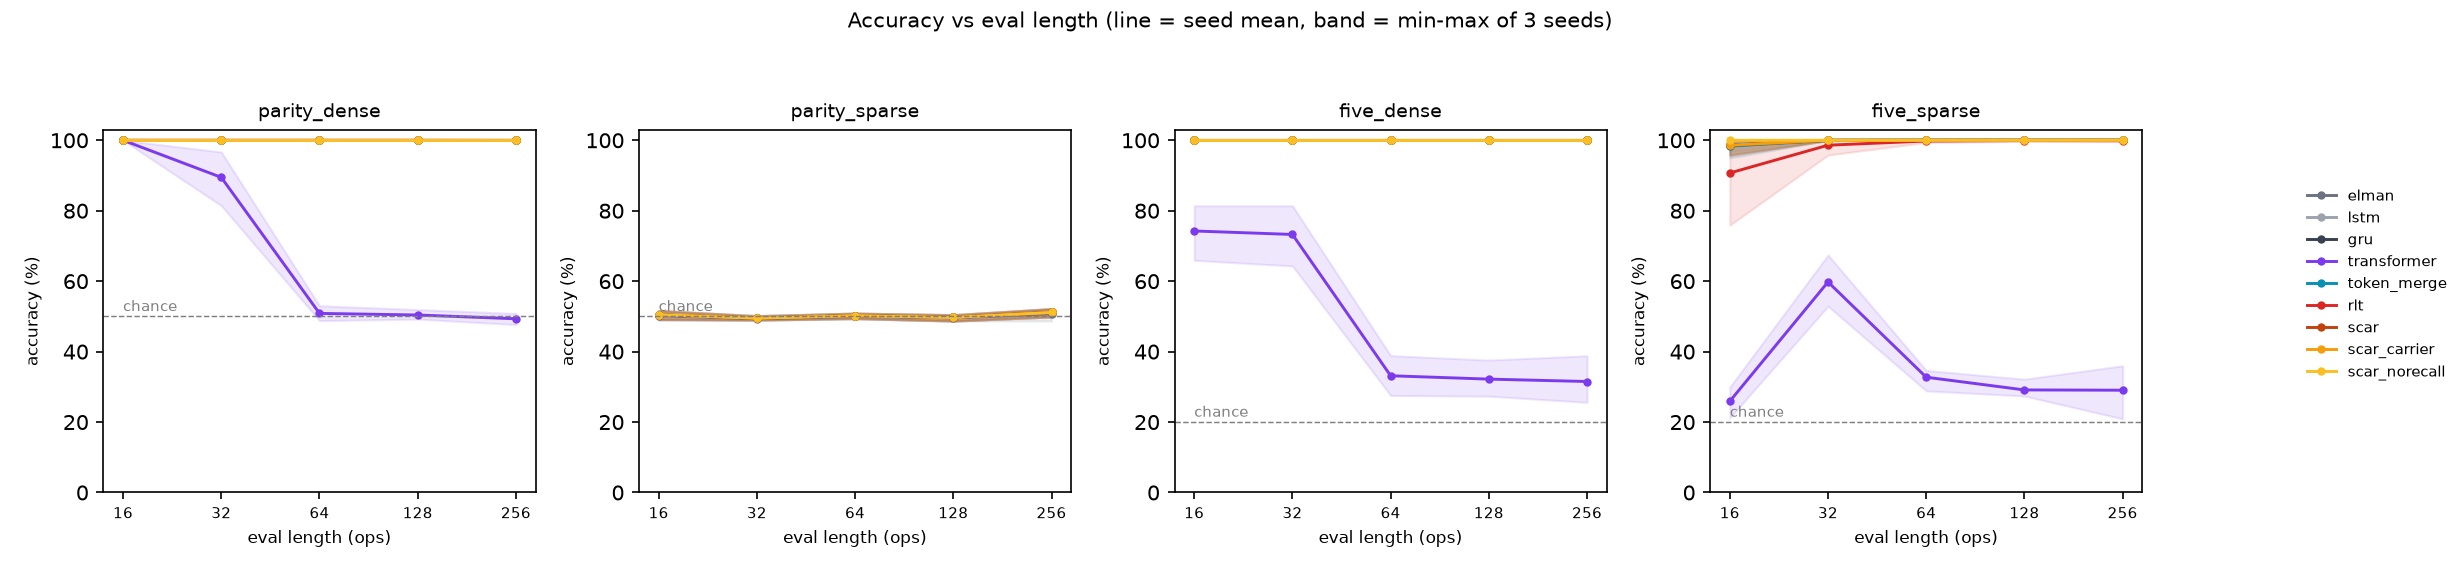
\includegraphics[width=\linewidth]{figures/accuracy_by_config.png}
\caption{Accuracy versus evaluation length. Lines are seed means and shaded bands span the three-seed minimum and maximum.}\label{fig:accuracy}
\end{figure}

\begin{table}[t]
\centering\small
\caption{Extrapolation accuracy (\%) at the longest evaluated length (parity/five: 256 operations; recall: 512 operations). No model was trained at these lengths.}\label{tab:extrap}
\resizebox{\linewidth}{!}{%
\begin{tabular}{l r c c c c c }
\toprule
Model & Params & parity dense & parity sparse & five dense & five sparse & recall sparse \\
\midrule
Elman RNN & 76,416 & 100.0\,$\pm$\,0.0 & 50.7\,$\pm$\,1.8 & 100.0\,$\pm$\,0.0 & 100.0\,$\pm$\,0.0 & 12.3\,$\pm$\,1.9 \\
LSTM & 75,648 & 100.0\,$\pm$\,0.0 & 51.1\,$\pm$\,1.2 & 100.0\,$\pm$\,0.0 & 100.0\,$\pm$\,0.0 & 12.6\,$\pm$\,1.7 \\
GRU & 77,280 & 100.0\,$\pm$\,0.0 & 51.1\,$\pm$\,1.2 & 100.0\,$\pm$\,0.0 & 100.0\,$\pm$\,0.0 & 56.6\,$\pm$\,18.5 \\
Transformer (full causal) & 76,608 & 49.3\,$\pm$\,1.6 & 51.1\,$\pm$\,1.2 & 31.5\,$\pm$\,6.7 & 29.0\,$\pm$\,7.6 & 77.5\,$\pm$\,19.7 \\
TokenMerge (RLT abl.) & 82,880 & 100.0\,$\pm$\,0.0 & 51.1\,$\pm$\,1.2 & 100.0\,$\pm$\,0.0 & 100.0\,$\pm$\,0.0 & 8.1\,$\pm$\,7.0 \\
RLT & 75,000 & 100.0\,$\pm$\,0.1 & 51.1\,$\pm$\,1.2 & 100.0\,$\pm$\,0.0 & 99.9\,$\pm$\,0.2 & 100.0\,$\pm$\,0.0 \\
SCAR & 77,896 & 100.0\,$\pm$\,0.0 & 51.1\,$\pm$\,1.2 & 100.0\,$\pm$\,0.0 & 100.0\,$\pm$\,0.0 & 100.0\,$\pm$\,0.0 \\
SCAR-carrier (no memory) & 77,280 & 100.0\,$\pm$\,0.0 & 51.1\,$\pm$\,1.2 & 100.0\,$\pm$\,0.0 & 100.0\,$\pm$\,0.0 & 56.6\,$\pm$\,18.5 \\
SCAR-no-recall & 78,710 & 100.0\,$\pm$\,0.0 & 51.1\,$\pm$\,1.2 & 100.0\,$\pm$\,0.0 & 100.0\,$\pm$\,0.0 & 30.5\,$\pm$\,32.4 \\
\bottomrule
\end{tabular}}
\end{table}

\subsection{Delayed recall and ablations}
At the trained length, the models that clearly beat the 12.5\% chance floor are GRU, Transformer (full causal), TokenMerge (RLT abl.), RLT, SCAR, SCAR-carrier (no memory), SCAR-no-recall. The more revealing comparison is extrapolation: at 512 operations, SCAR remains at 100.0\,$\pm$\,0.0\%, while the carrier-only and no-recall variants fall to 56.6\,$\pm$\,18.5\% and 30.5\,$\pm$\,32.4\%, respectively.
\begin{figure}[t]
\centering
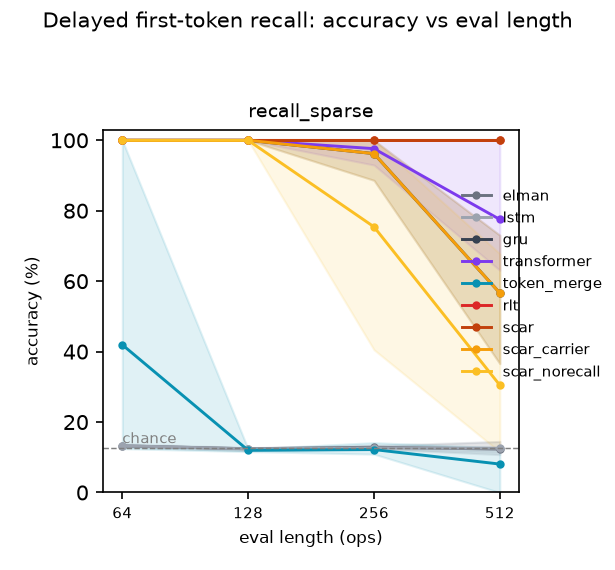
\includegraphics[width=\linewidth]{figures/recall_curves.png}
\caption{Delayed first-token recall across evaluation lengths; chance is 12.5\%.}\label{fig:recall}
\end{figure}

The two ablations are parameter-matched to SCAR within roughly one percent: SCAR-carrier widens the GRU carrier to d=112 after removing the memory, while SCAR-no-recall widens d to 98 while retaining the write path. Both reach 100.0\,$\pm$\,0.0\% at the trained recall length, so neither component is required to fit the short training distribution. At 512 operations, however, the full model reaches 100.0\,$\pm$\,0.0\% versus 56.6\,$\pm$\,18.5\% without memory and 30.5\,$\pm$\,32.4\% without the read path. This supports a narrow conclusion: constant-size memory is useful for long-delay extrapolation in this probe, but the experiment does not show that the memory improves every task or every length.
\begin{figure}[t]
\centering
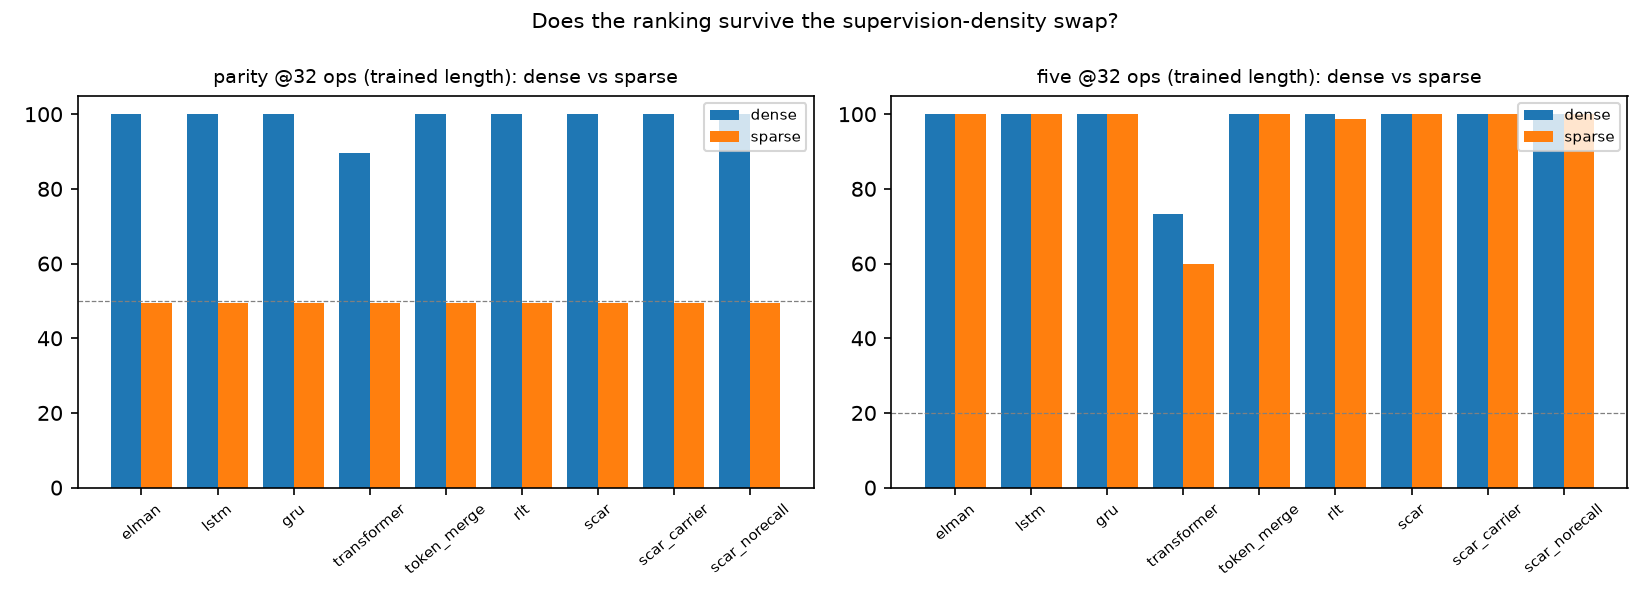
\includegraphics[width=\linewidth]{figures/density_swap.png}
\caption{Changing supervision density changes which architectures escape chance on the trained-length parity and five-state tasks.}\label{fig:density}
\end{figure}


\section{Study 2: stress tests and failure modes}
The preregistered follow-up separates the original recall headline from stress tests of length, training context, retrieval type, capacity, and memory intervention. At 4,096 operations, the recall-length sweep gives the following descriptive endpoint comparison; the model was trained at only 64 operations.
\begin{table}[t]
\centering\small
\caption{Study 2A delayed-recall accuracy at 4,096 operations; models were trained at 64 operations. Mean$\pm$std over five seeds.}\label{tab:study2-recall}
\begin{tabular}{l c}
\toprule
Model & Accuracy (\%) \\
\midrule
GRU & 13.4\,$\pm$\,0.6\% \\
LSTM & 12.7\,$\pm$\,0.3\% \\
Transformer (full causal) & 23.3\,$\pm$\,21.9\% \\
RLT & 97.4\,$\pm$\,5.7\% \\
SCAR & 72.8\,$\pm$\,13.8\% \\
SCAR-carrier (no memory) & 13.4\,$\pm$\,0.6\% \\
SCAR-no-recall & 12.5\,$\pm$\,0.4\% \\
\bottomrule
\end{tabular}
\end{table}
The train/test ratio probes show SCAR at 100.0\,$\pm$\,0.0\% when trained at 32 operations and 12.2\,$\pm$\,0.8\% when trained at 128 operations, so the 512-token result is not treated as a universal context-length law. Associative recall is a useful negative control: SCAR reaches 11.4\,$\pm$\,0.6\% at 32 key/value pairs against a 6.25\% single-choice chance floor, indicating that the fixed exponential summaries do not solve arbitrary multi-item retrieval.

Selective copy makes the retrieval target multi-output rather than a single first-token label. At 32 marked items, SCAR's free-running exact-sequence accuracy is 0.0\,$\pm$\,0.0\% under the high-entropy distractor condition and 0.0\,$\pm$\,0.0\% under the low-entropy condition. The slot sweep's 512-operation SCAR endpoints are 1: 91.1\%, 2: 100.0\%, 4: 77.1\%, 8: 86.7\%, 16: 100.0\%, 32: 100.0\%, 64: 89.1\%. Frozen-memory interventions at 512 operations are equalize 100.0\%, fastest 100.0\%, noise 60.4\%, shuffle 100.0\%, slowest 100.0\%. The learned multi-timescale decay sweep ended with final slot half-lives spanning 8.1--470.1 operations across the 16 slots, with mean read-attention entropy 2.70. These are exploratory, descriptive comparisons; no significance claim is made from the small seed counts. The persistent-state accounting is constant for SCAR across the tested lengths (5,984 bytes at 4,096 operations), compared with 3,281,920 bytes for RLT-lite and 5,505,024 bytes for the full causal Transformer at that endpoint. This counts streaming state, not parameter storage or transient training activations.
\begin{table}[t]
\centering\small
\caption{Persistent inference state in bytes, excluding parameters and transient training activations. Values are generated from the model state accounting.}\label{tab:state-memory}
\begin{tabular}{l r r r}
\toprule
Model & 64 & 512 & 4,096 \\
\midrule
GRU & 448 & 448 & 448 \\
RLT & 56,320 & 414,720 & 3,281,920 \\
SCAR & 5,984 & 5,984 & 5,984 \\
Transformer (full causal) & 86,016 & 688,128 & 5,505,024 \\
\bottomrule
\end{tabular}
\end{table}
\begin{figure}[t]
\centering
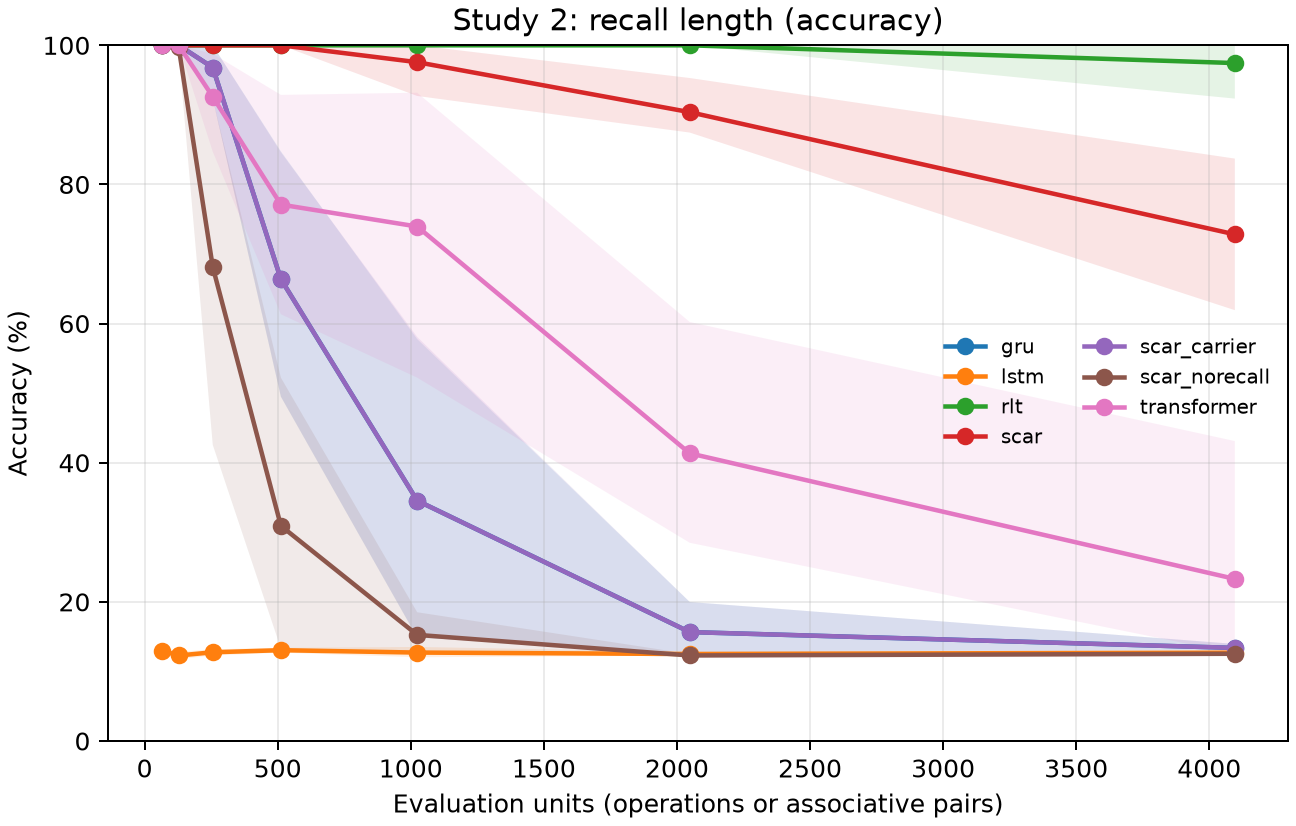
\includegraphics[width=\linewidth]{figures/study2_recall_length_accuracy.png}
\caption{Study 2A: delayed-recall accuracy through 4,096 operations after training at 64 operations. Shaded bands are bootstrap intervals over seed means.}\label{fig:study2-recall}
\end{figure}
\begin{figure}[t]
\centering
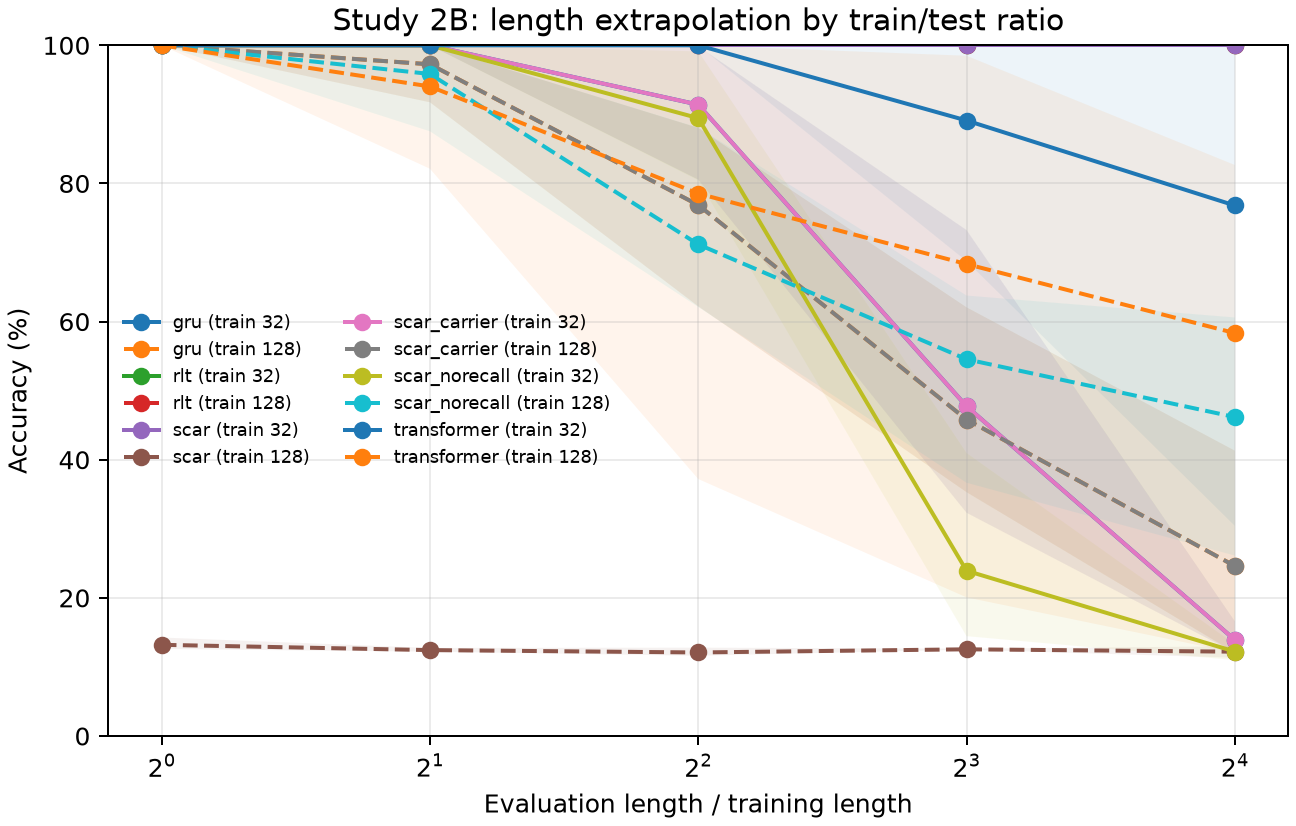
\includegraphics[width=\linewidth]{figures/study2_ratio_comparison.png}
\caption{Study 2B: accuracy plotted against evaluation length divided by training length for two training contexts.}\label{fig:study2-ratio}
\end{figure}
\begin{figure}[t]
\centering
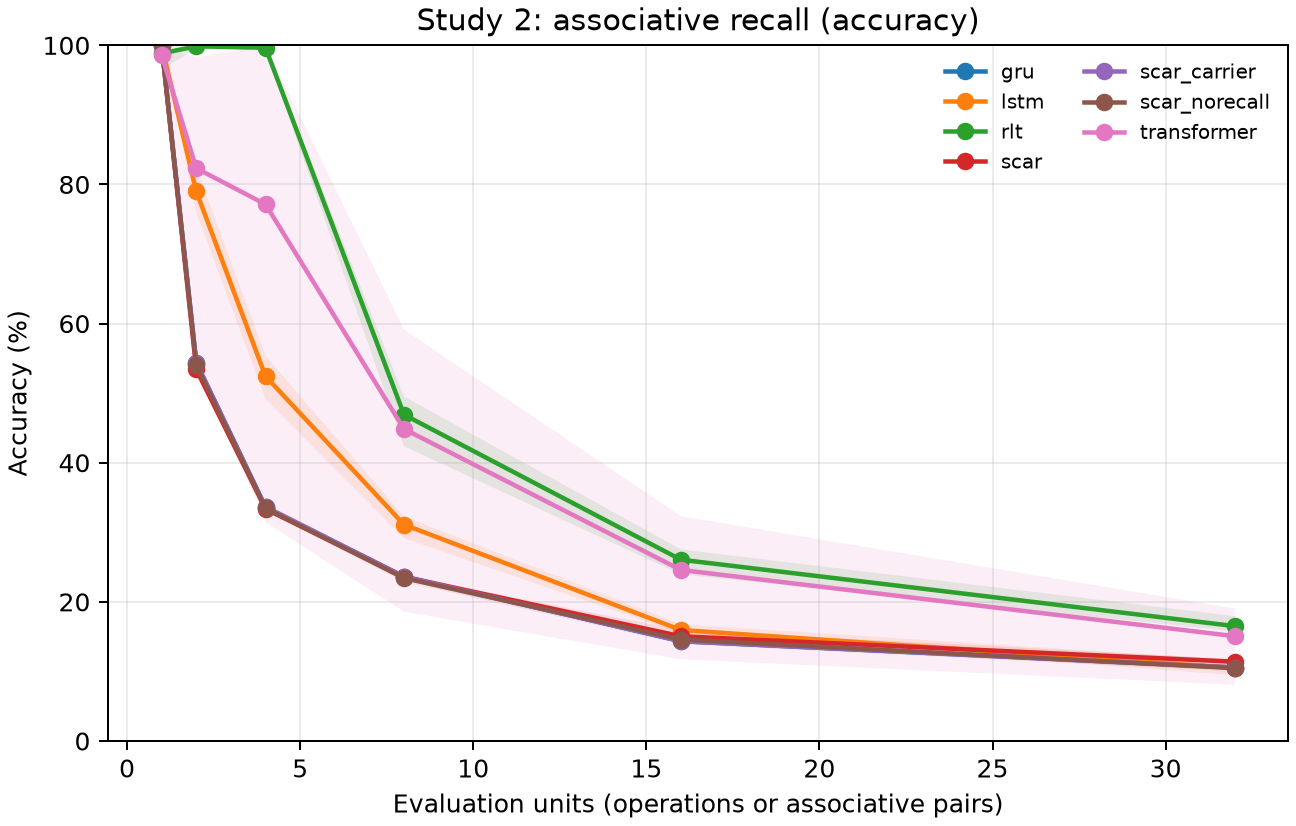
\includegraphics[width=\linewidth]{figures/study2_associative_recall_accuracy.png}
\caption{Study 2C: associative key/value recall across the number of presented pairs. Shaded bands are bootstrap intervals over seed means.}\label{fig:study2-associative}
\end{figure}
\begin{figure}[t]
\centering
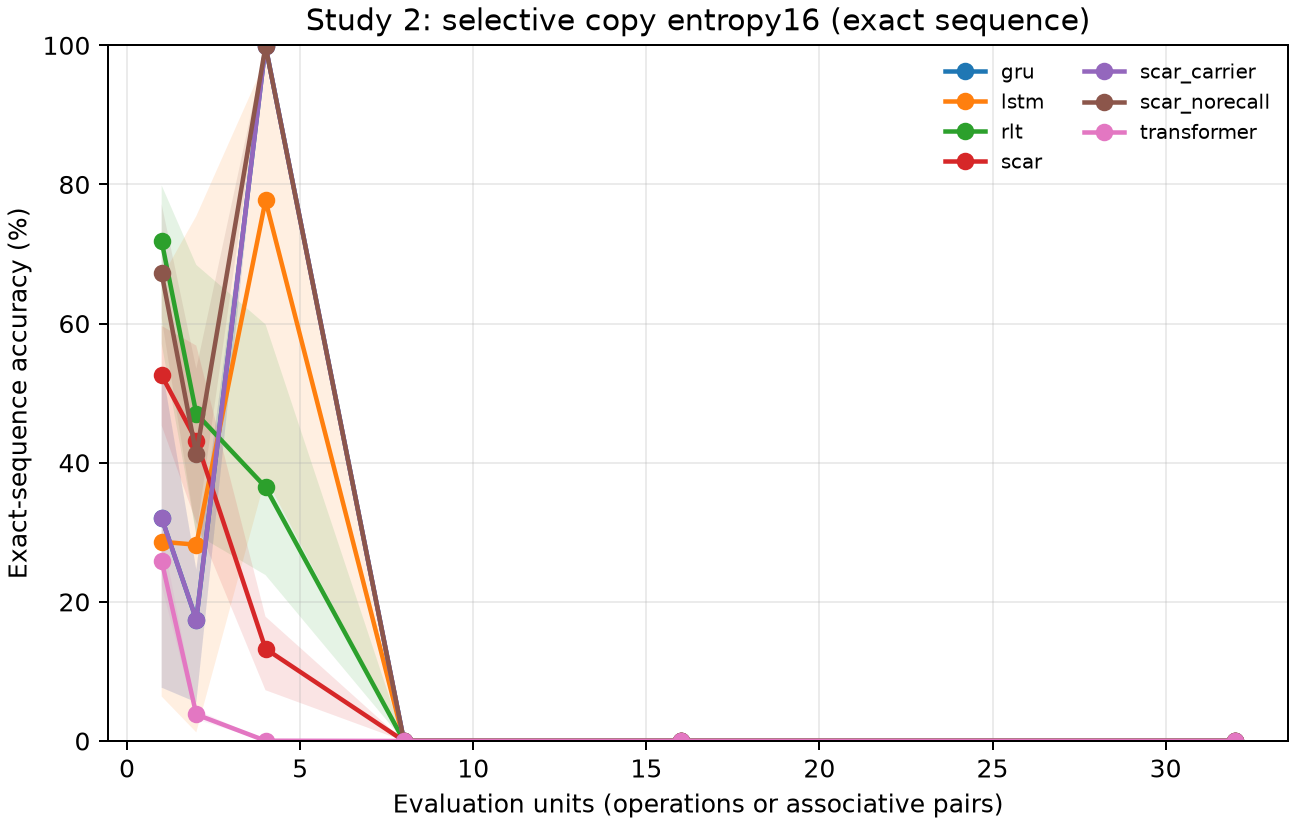
\includegraphics[width=\linewidth]{figures/study2_selective_copy_entropy16_exact_sequence.png}
\caption{Study 2D: free-running exact-sequence accuracy for high-entropy selective copy.}\label{fig:study2-copy}
\end{figure}
\begin{figure}[t]
\centering
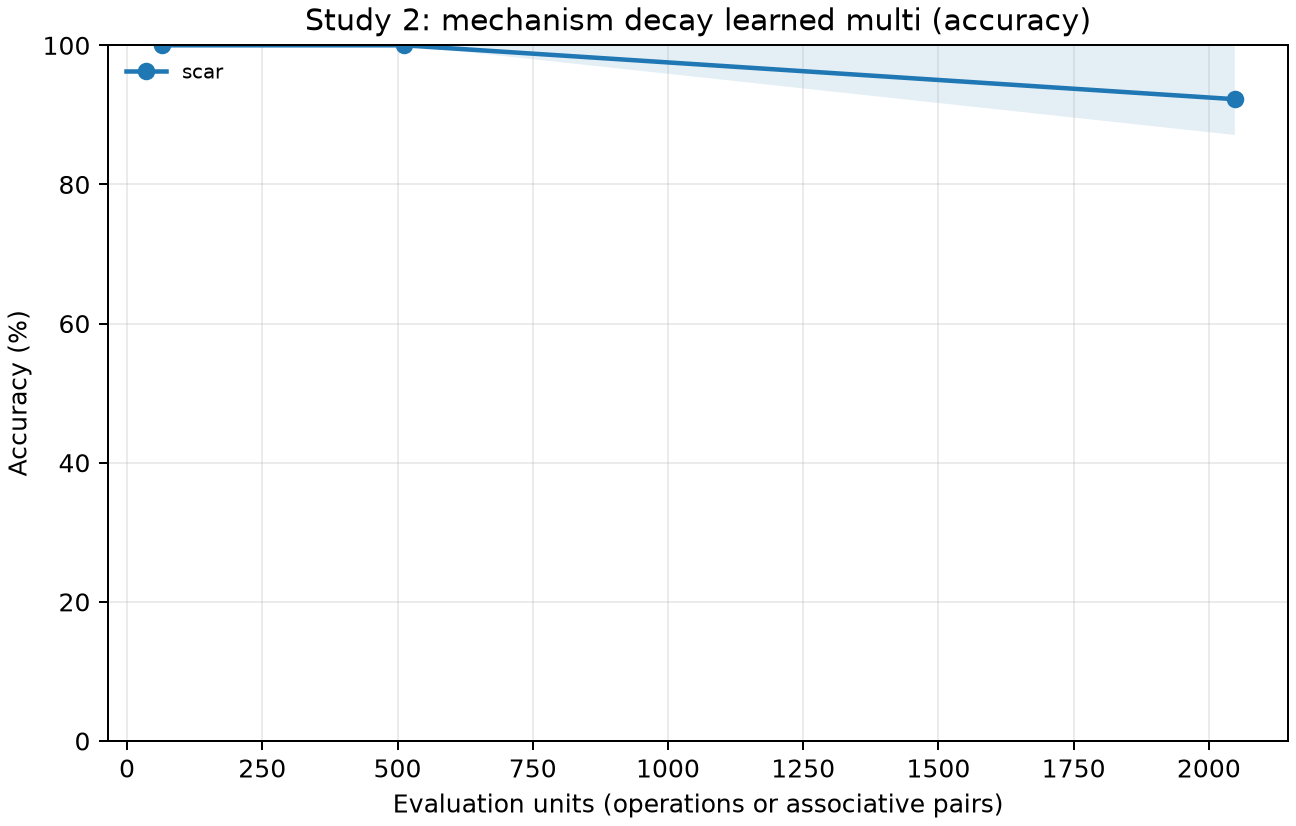
\includegraphics[width=\linewidth]{figures/study2_mechanism_decay_learned_multi_accuracy.png}
\caption{Study 2E: accuracy for the learned multi-timescale decay mechanism variant.}\label{fig:study2-mechanism}
\end{figure}
\begin{figure}[t]
\centering
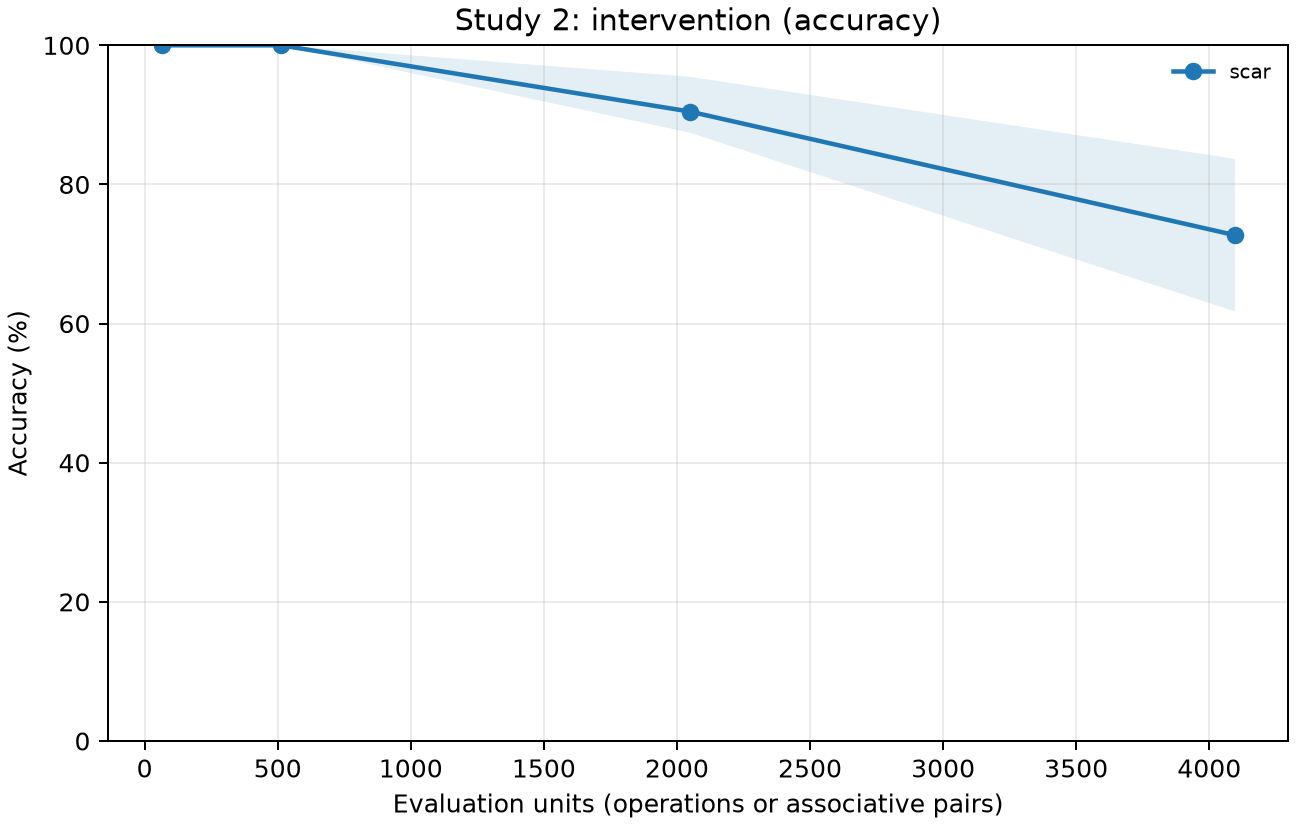
\includegraphics[width=\linewidth]{figures/study2_intervention_accuracy.png}
\caption{Study 2F: frozen-memory intervention accuracy at the tested evaluation contexts.}\label{fig:study2-intervention}
\end{figure}


\clearpage

\section{Compute cost}
\begin{table}[t]
\centering\small
\caption{Dedicated serial cost benchmark: 100 timed iterations after 20 warmup, torch threads = 2, batch 64, train length 32+BOS, inference length 128+BOS. Median [min--max] ms.}
\label{tab:cost}
\resizebox{\linewidth}{!}{%
\begin{tabular}{l l c l}
\toprule
Model & train ms/step & $\times$GRU & infer ms/batch \\
\midrule
Elman RNN & 23.3 [22.3--27.5] & 0.75$\times$ & 29.3 \\
LSTM & 29.9 [28.7--47.2] & 0.96$\times$ & 36.3 \\
GRU & 31.0 [30.0--46.8] & 1.00$\times$ & 33.2 \\
Transformer (full causal) & 32.6 [31.6--35.2] & 1.05$\times$ & 102.5 \\
TokenMerge (RLT abl.) & 217.6 [206.5--249.9] & 7.03$\times$ & 257.1 \\
RLT & 243.7 [236.2--280.8] & 7.87$\times$ & 391.9 \\
SCAR & 96.5 [92.6--127.0] & 3.12$\times$ & 104.8 \\
SCAR-carrier (no memory) & 32.2 [31.2--41.1] & 1.04$\times$ & 33.7 \\
SCAR-no-recall & 43.4 [42.4--63.4] & 1.40$\times$ & 64.7 \\
\bottomrule
\end{tabular}}
\end{table}

On this CPU, full SCAR costs 3.12$\times$ a GRU per training step, while the carrier-only ablation costs 1.04$\times$. SCAR is 0.40$\times$ the measured RLT training-step cost. This falsifies the original ~1$\times$-GRU cost target while supporting a substantial reduction relative to RLT. These are controlled single-machine timings, not hardware-independent complexity claims.
\begin{figure}[t]
\centering
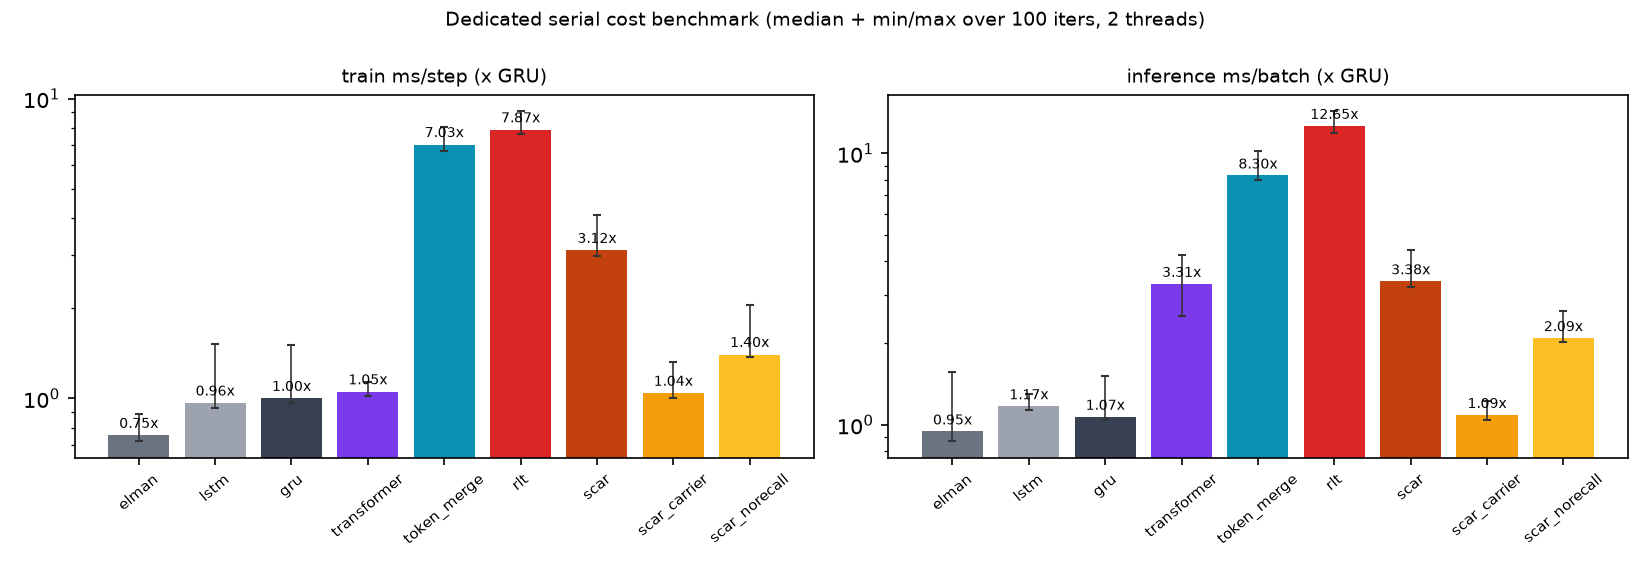
\includegraphics[width=\linewidth]{figures/cost.png}
\caption{Dedicated serial CPU benchmark. Bars show medians and whiskers show the repeated-iteration minimum and maximum.}\label{fig:cost}
\end{figure}


\section{Discussion}
The clean fixed-length density comparison is descriptive: Under sparse parity supervision, 9 of nine architectures remain at the 50\% chance floor (Elman RNN, LSTM, GRU, Transformer (full causal), TokenMerge (RLT abl.), RLT, SCAR, SCAR-carrier (no memory), SCAR-no-recall). Dense supervision makes almost every architecture look successful, whereas sparse parity leaves several at chance. With only three seeds, we report means and sample standard deviations but do not call near-equal cells significance-labeled. The strongest result is therefore not that SCAR universally wins: it is that the parameter-matched carrier-only model can match SCAR on short tasks while losing its long-delay advantage.

The combined evidence supports a conditional claim. At trained lengths, the
parameter-matched SCAR ablations often fit as well as the full model; at 4,096
operations, full SCAR retains a large advantage over those ablations, although
RLT remains stronger in that endpoint comparison. Study 2 also marks the
boundary of the benefit rather than assuming that one-token recall implies
general-purpose memory: associative retrieval is only modestly above chance,
free-running selective copy collapses at 32 items, and the mechanism and
frozen-state interventions are descriptive rather than a causal decomposition.
Dense versus sparse supervision remains a methodological confounder when the
protocol is not held fixed, so we do not present a universal architecture
ranking or a significance claim from three seeds.

\section{Limitations}
This is a synthetic study with small models, a single parameter scale, three
seeds for most Study 2 families, and short training budgets. The tasks test
exact state tracking rather than natural-language modeling, multimodal
reasoning, or noisy real-world sequences. Associative and selective-copy
tasks probe more than first-token recall but do not establish language-model
quality. The ablations are parameter-matched, but changing width to replace
removed modules can itself change optimization and representation capacity.
The RLT comparison is a small implementation, not a claim about the behavior
of all RLT variants. Timing uses one CPU machine, two PyTorch threads, a
parity-sized vocabulary, and an unoptimized research implementation; measured
ratios should not be generalized to GPU kernels or production runtimes.
Finally, the fixed memory's success on this recall generator does not establish
that learned exponential summaries are sufficient for arbitrary long-context
tasks.

\section{Reproducibility and release}
The repository contains the model and task code (``bench.py``), regression
tests (``tests/``), the quarantined Study 1 artifacts, all collected Study 2
JSON files and manifests, aggregation and chart scripts, the generated tables,
and the figures used in this PDF. All optimizer steps and training timings in
the two studies run on Kaggle CPU kernels through ``kaggle/``; no local
training is required.
The release command sequence is:
\begin{verbatim}
python3 -m pytest tests/ -q
python3 aggregate.py
python3 make_charts.py
python3 -m study2.analyze study2_results --out analysis/study2
python3 study2/state_memory.py --out analysis/study2/state_memory.json
python3 make_paper.py
(cd paper && tectonic paper.tex)
\end{verbatim}
The generated summary includes per-seed values and the curriculum flag so the
reported condition cannot silently drift from the trained artifacts.

\begin{thebibliography}{12}
\bibitem{elman1990}
J. L. Elman, ``Finding structure in time,'' \emph{Cognitive Science},
14(2), 179--211, 1990. doi:10.1207/s15516709cog1402\_1.

\bibitem{hochreiter1997}
S. Hochreiter and J. Schmidhuber, ``Long short-term memory,''
\emph{Neural Computation}, 9(8), 1735--1780, 1997.

\bibitem{cho2014}
K. Cho et al., ``Learning phrase representations using RNN encoder--decoder
for statistical machine translation,'' arXiv:1406.1078, 2014.

\bibitem{vaswani2017}
A. Vaswani et al., ``Attention is all you need,''
\emph{Advances in Neural Information Processing Systems}, 30, 2017.
arXiv:1706.03762.

\bibitem{sukhbaatar2015}
S. Sukhbaatar, J. Weston, R. Fergus, et al., ``End-to-end memory networks,''
\emph{Advances in Neural Information Processing Systems}, 28, 2015.
arXiv:1503.08895.

\bibitem{gu2022s4}
A. Gu, K. Goel, and C. Ré, ``Efficiently modeling long sequences with
structured state spaces,'' in \emph{International Conference on Learning
Representations}, 2022. arXiv:2111.00396.

\bibitem{mikolov2015longmemory}
T. Mikolov, A. Joulin, S. Chopra, M. Mathieu, and M. Ranzato,
``Learning longer memory in recurrent neural networks,'' arXiv:1412.7753, 2015.

\bibitem{katharopoulos2020linear}
A. Katharopoulos, A. Vyas, N. Pappas, and F. Fleuret,
``Transformers are RNNs: Fast autoregressive transformers with linear attention,''
in \emph{International Conference on Machine Learning}, 2020. arXiv:2006.16236.

\bibitem{sun2023retnet}
Y. Sun et al., ``Retentive network: A successor to Transformer for large
language models,'' arXiv:2307.08621, 2023.

\bibitem{gu2024mamba}
A. Gu and T. Dao, ``Mamba: Linear-time sequence modeling with selective state
spaces,'' arXiv:2312.00752, 2023.

\bibitem{dai2019transformerxl}
Z. Dai, Z. Yang, Y. Yang, J. Carbonell, Q. V. Le, and R. Salakhutdinov,
``Transformer-XL: Attentive language models beyond a fixed-length context,''
\emph{Proceedings of ACL}, 2019. arXiv:1901.02860.

\bibitem{rae2020compressive}
J. W. Rae, A. Potapenko, S. M. Jayakumar, and T. P. Lillicrap,
``Compressive transformers for long-range sequence modelling,'' in
\emph{International Conference on Learning Representations}, 2020.
arXiv:1911.05507.

\bibitem{arora2023zoology}
S. Arora, S. Eyuboglu, A. Timalsina, I. Johnson, M. Poli, J. Zou,
A. Rudra, and C. Ré, ``Zoology: Measuring and improving recall in efficient
language models,'' arXiv:2312.04927, 2023.

\bibitem{zhang2026rlt}
Y. Zhang, J. Feng, and S. Qin, ``Recurrent Looped Transformer,'' technical
report, 2026. \url{https://github.com/yifanzhang-pro/recurrent-looped-tranformer}.
\end{thebibliography}
\end{document}
